\section{Устойчивость}
Исследуем на устойчивость систему $\dot{x} = Ax$, где $A \in \mathbb{R}^{nxn}$ и $\Re{\lambda_j} \neq 0$. Введем функцию $\chi(\lambda) = \left|\lambda I - A\right| = \lambda^n+C_{n-1} + \cdots + C_1 \lambda + C_0 = (\lambda - \lambda_1)\cdot \cdots \cdot (\lambda - \lambda_n)$. Проблема в том, что все собственные значения  сложно искать
\begin{definition}
	Матрица $A$ - усточива $\Leftrightarrow \forall j \Re{\lambda_j} < 0$. 
	Матрица $A$ - неусточива $\Leftrightarrow \exists j \Re{\lambda_j} > 0$. 	
\end{definition}
$\chi(\lambda) = 0$ --- критерий асимптотической устойчивости.\\
$A$ --- устойчива $\Rightarrow \chi(0) = C_0 > 0$. Заметим, что $\chi(0) = \prod_{j=1}^{n}\left(-\lambda_j\right)$. В случае действительного $\lambda_j$ получаем $-\lambda_j  > 0$, а в комплексном случае получим $(-\lambda_j)(-\overline{ \lambda_j }) = |\lambda_j|^2=(\alpha^2+\beta^2)>0$\\
\subsection{графический метод исследования на устойчивость} 
Рассмотрим $\lambda = i \omega$. Заметим, что тогда $\overline{\chi}(i\omega) = \chi(i\omega)$
Тогда получим:
\begin{equation*}
\chi(i \omega) = (i \omega - \lambda_1)\cdot \cdots \cdot (i \omega - \lambda_n)
\end{equation*}
Тогда возможны два случая: \\
\begin{center}
	\begin{tabular}{cc}
		$\Real{\lambda_j} < 0$ & $\Real{\lambda_j} > 0$\\
		$\Arg{i \omega - \lambda_i} \bigg|_{w = - \infty}^{+\infty}\bigg.	= \pi$ & $\Arg{i \omega - \lambda_i} \bigg|_{w = - \infty}^{+\infty}\bigg.	= -\pi$
	\end{tabular}
\end{center}
Тогда получим критерий асимптотической устойчивости Михайлова:\\
$\Arg{\chi(i \omega)}\bigg|_{\omega = 0}^{+\infty} = \frac{\pi}{2} n \Leftrightarrow \forall j \Real{\lambda_j} < 0$.\\
Иначе критерий Михайлова можно воспринимать как количество четвертей пройденных графиком $\chi(i\omega)$ или годографом по $\omega \in \mathbb{R}^+$ 
\begin{figure}[H]
	\center{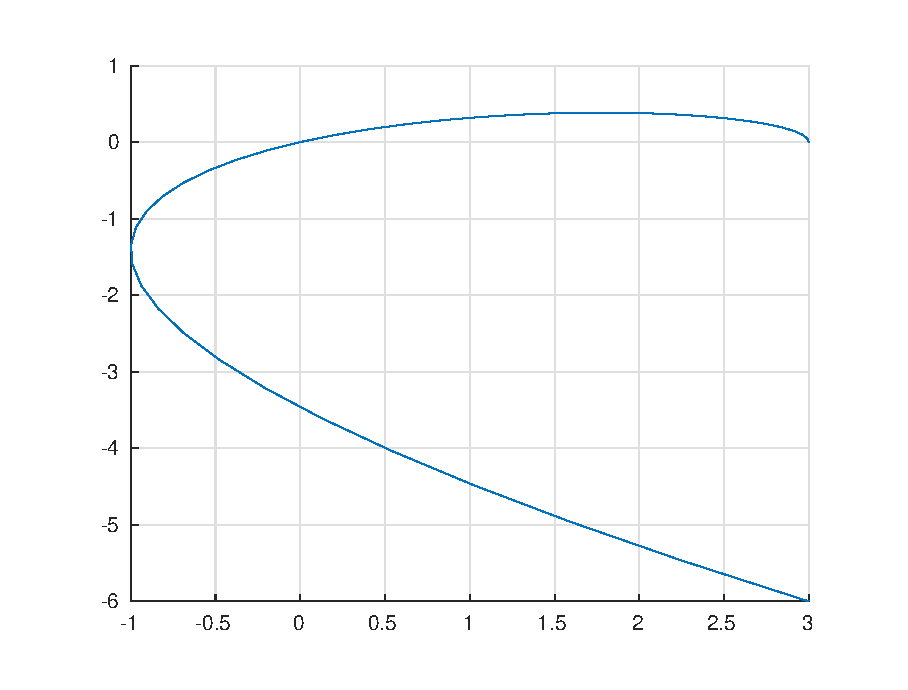
\includegraphics[width=0.6\textwidth]{ch15/godograph.eps}}
	\caption{ Пример годографа с $\chi(\lambda) = \lambda^4+\lambda^3+4\lambda^2+\lambda+3$}
\end{figure}
\subsection{Применение к теории управления}
\subsection{Теорема Найквиста}
Пусть $H$ имеет $q$ неустойчивых полюсов и $n-q$ устойчивых (не имеет чисто мнимых). Тогда замкнутая система устойчива тогда и только тогда когда $H(i \omega)$ не проходит через $-1$ и делает при $\omega = (0; +\infty)$ $\frac{q}{2}$ полных оборотов против часовой стрелки. 
\begin{figure}[H]
	\center{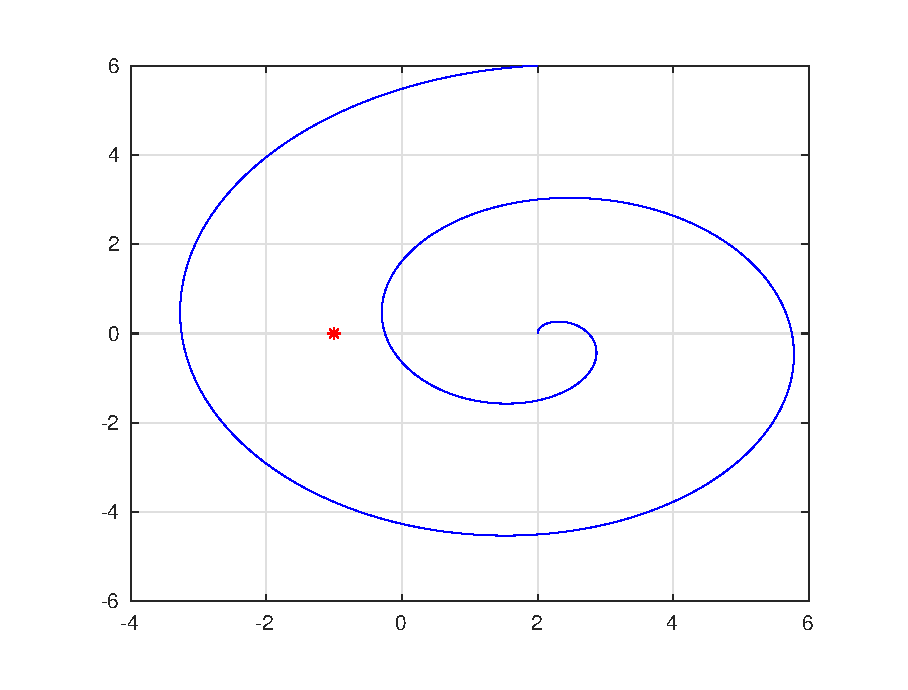
\includegraphics[width=0.6\textwidth]{ch15/naiq.eps}}
\end{figure}